% !TEX root = ../main.tex

\chapter{GNSS弹性功率机理与影响}

\section{GNSS弹性功率的定义}
\subsection{基本概念}
弹性功率是GNSS现代化进程中的一项重要能力,它允许卫星在不同信号分量之间重新分配其发射功率\cite{zhang2025analysis,xiang2020understanding}。这种可编程的功率输出能力旨在增强特定信号的强度,以更好地满足作战需求或提高抗干扰性能\cite{liu2024characteristics,esenbuga2020impact,esenbuuga2020impact,zhang2025analysis}。

弹性功率的核心在于在不增加卫星总发射功率的前提下,通过转移功率来提高某些信号的标称发射功率\cite{zhang2025analysis}。其主要目的是提升信号的抗干扰能力,保护如美国国防部及其盟友等军事用户在国家安全受威胁时仍能使用GPS,并通过增强军事P(Y)和M码信号的强度来实现这一目标\cite{jimenez2010measured,zhang2025analysis}。

弹性功率通过调整信号的调制方式,将功率从一个信号分量转移到另一个分量。例如,GPS卫星可以在L1/L2频段上,将M码的功率转移到P(Y)码上,从而增加P(Y)码的功率\cite{zhang2025analysis}。然而,这种功率重新分配并不能同时增加所有信号分量的发射功率\cite{esenbuuga2020impact,esenbuga2020impact}。根据2021年发布的GPS 接口规范 IS-GPS-200M,Block IIR-M和IIF卫星的单个信号分量在开启弹性功率后,其功率输出可能超过预设的最大值,但预计不会超过-150 dBW\cite{zhang2025analysis,esenbuuga2020impact,esenbuga2020impact,ISGPS200M2021}。

\subsection{发展历程}
GNSS系统中,GPS和BDS均配备了弹性功率功能。GPS方面,Block IIR-M(7颗)、 Block IIF(12 颗)具备弹性功率能力。BDS则是在BDS-2卫星配备了弹性功率功能,其机制与GPS类似,能够调整发射功率以提升抗干扰能力\cite{liu2024characteristics,lu2025new,liu2025effects}。GPS的首次弹性功率演示发生在2010年9月7日至12日,当时提高了L1和L2信号的P(Y)码功率,并被认为是成功的\cite{jimenez2010measured,zhang2025analysis}。自2017年1月起,GPS在大部分Block IIF卫星上启动了区域性弹性功率增强\cite{esenbuga2020impact,zhang2025analysis}。在2018年4月,GPS还进行了全球性的弹性功率开启(4月13日至17日,为期四天)和另一次区域性事件(4月底,为期三天)\cite{xiang2020understanding,zhang2025analysis}。2020年2月14日之后,GPS实施了新的弹性功率模式(模式4-9),其对L1和L2 P(Y)码信号同时产生影响,并表现出不同的地面覆盖范围。这些后期模式对Hatch–Melbourne–Wübbena(HMW)组合和轨道确定的影响更为显著\cite{zhang2024improved}。BDS--2卫星在2020-2023年期间共发生了九次弹性功率事件,其中倾斜地球同步轨道(Inclined Geosynchronous Orbit,IGSO)卫星最为频繁开启\cite{liu2025effects}。
\section{弹性功率的模式特征与可视化}
截至目前,GPS 卫星的弹性功率共有 10 种模式(Mode 1 至 Mode 10),覆盖了从 2017 年到 2023 年的多个时间段,每种模式对应不同的激活时间段、卫星、区域和信号强度变化,如表 \ref{tab:flex_power_modes} 所示。

不同模式对应的开启中心位置不同,有单中心、双中心和三中心配置,也存在在两根经线中间的区域全部开启的配置。不同模式下对于不同频点信号强度的增强也存在差异。一般情况下,L1C、S1W、S2W 三个频点在弹性功率开启期间只有一至两个频点存在信号强度增强,同时可能存在另外的信号强度减弱,如 Mode 3 的 S1W、S2W 频点增强了 9-11dB,对应 L1C 频点信号强度减弱了 2-3dB。由于 GPS 系统中军用 M 码信号无法获得,因此无法得到完整的信号重新分配规则。

不同模式开启的中心与覆盖区域可以通过卫星轨迹在二维地图上的轨迹来表示。
以 2020 年 2 月 15 日开启的弹性功率 Mode~4 为例,其开启区域如图\ref{fig:mode4track}所示。
其中,红色十字与黄色十字分别表示两个弹性功率开启中心,
由黄色线段与红色线段共同围绕形成的深色区域为弹性功率开启区域。
如果将该平面世界地图投影到三维球体上,可以得到图\ref{fig:3dtrack}。
从图\ref{fig:3dtrack}中可以发现,由黄色线段与红色线段围成的区域在投影到三维球体后,
实际得到的是两个分别以黄色十字和红色十字为中心的圆形投影区域,
而弹性功率开启区域则为这两个圆形区域取并集后形成的深色区域。在弹性功率功能区域激活后,当具备功能的卫星投影进入对应区域后,便会开启弹性功率增强功能。

\begin{figure}
    \centering
    \includegraphics[width=1\linewidth]{figures/c2/mode4track.png}
    \bicaption{弹性功率开启区域二维地图示意图}{Two-dimensional schematic map of the flex power activation region.}
    \label{fig:mode4track}
\end{figure}

\begin{figure}
    \centering
    \includegraphics[width=1\linewidth]{figures/c2/3dtrack.png}
    \bicaption{弹性功率开启区域三维地图示意图}{Three-dimensional schematic map of the flex power activation region.}
    \label{fig:3dtrack}
\end{figure}


\begin{table}[htbp]
\centering
\bicaption{各类弹性功率模式及其特征\cite{esenbuuga2023recent}}{Various flex power modes and their characteristics.\cite{esenbuuga2023recent}}
\label{tab:flex_power_modes}
\small % 略微缩小字号以适应更多内容
\begin{tabularx}{\textwidth}{@{} p{1.3cm} p{1.5cm} p{2.5cm} X p{1.2cm} p{1cm} p{1cm} p{1cm} @{}}
\toprule
\textbf{模式} &
\textbf{型号} &
\textbf{DOY/Year} &
\textbf{开启中心} &
\textbf{中心数} &
\textbf{L1C} &
\textbf{S1W} &
\textbf{S2W} \\
\midrule
Mode 1 & IIF & 027/2017--044/2020 & 41$^\circ$E / 37$^\circ$N & 单中心 & 2.5 & 2.5 & -- \\
Mode 2 & IIR-M/IIF & 103--107/2018; 151--155/2021; 254--257/2021; 266--267/2021; 296/2021; 299/2021; 320/2021 & 全球 & 无中心 & -- & 6 & 5 \\
Mode 3 & IIR-M/IIF & 117,121,124/2018; 171--172/2019 & 115$^\circ$W / 40$^\circ$N & 单中心 & --(2-3) & 9--11 & -- \\
Mode 4 & IIR-M/IIF & 045--103/2020 & 37$^\circ$E / 35$^\circ$N; 69$^\circ$E / 35$^\circ$N & 双中心 & -- & 6 & 5 \\
Mode 5 & IIR-M/IIF & 104--124/2020; 130--165/2020; 172--174/2020; 185--188/2020 & 37$^\circ$E / 35$^\circ$N; 69$^\circ$E / 35$^\circ$N & 双中心 & -- & 9--11 & -- \\
Mode 6 & IIR-M/IIF & 125--129/2020; 137--150/2021; 156--253/2021; 258--265/2021; 268--295/2021; 297--298/2021; 300--319/2021; 321/2021--059/2022 & 155$^\circ$E 至 30$^\circ$W & 无中心 & -- & 9--11 & -- \\
Mode 7 & IIR-M/IIF & 166--171/2020; 175--184/2020; 189--215/2020; 235--256/2020; 275--292/2020; 298--299/2020; 310--320/2020; 326/2020--011/2021; 016--064/2021; 122--136/2021 & 111$^\circ$W / 33$^\circ$N; 33$^\circ$E / 34$^\circ$N; 70$^\circ$E / 35$^\circ$N & 三中心 & -- & 9--11 & -- \\
Mode 8 & IIR-M/IIF & 216--234/2020; 293--297/2020; 300--309/2020; 012--015/2021; 065--121/2021 & 109$^\circ$W / 32$^\circ$N; 70$^\circ$E / 35$^\circ$N & 双中心 & -- & 9--11 & -- \\
Mode 9 & IIR-M/IIF & 321--325/2020 & 76$^\circ$W / 41$^\circ$N; 70$^\circ$E / 35$^\circ$N & 双中心 & -- & 9--11 & -- \\
Mode 10 & IIR-M/IIF & 127--131, 2023 & 120$^\circ$W / 36$^\circ$N; 5$^\circ$W / 40$^\circ$N; 53$^\circ$E / 42$^\circ$N & 三中心 & -- & -- & -- \\
\bottomrule
\end{tabularx}
\end{table}

\section{GNSS弹性功率对观测信号特性的影响}
美国空军太空司令部(Air Force Space Command,AFSPC)最初认为弹性功率对全球绝大多数用户无明显影响,只有少数老旧接收机可能受不利影响\cite{yang2022real}。然而,现有研究表明,这种发射端的操作在增强特定信号抗压制能力的同时,也会对 GNSS 的精密数据处理产生影响。从物理层面上看,弹性功率的激活直接引发生信号出现 2–11 dB 量级的阶跃式变化,并导致卫星通道硬件延迟发生漂移,进而引起DCB和相位偏差出现纳秒级甚至周级的系统性不连续\cite{liu2024characteristics}。这些未被模型化的偏差若不经特殊处理,将向用户端传播,导致 PPP 收敛时间延长、PPP-AR 残差恶化,并限制 GNSS-R 反演及精密定轨等衍生应用的精度\cite{du2024effects,liu2024characteristics,wu2024effects,Wang2022A}。对于高精度定位用户而言,C/N0 的波动直接表征了信号的跟踪质量与功率模式,而 DCB 的稳定性则决定了伪距校正与电离层建模的精度\cite{steigenberger2019flex}。因此,本节将重点对弹性功率在 C/N0 及 DCB 上的具体影响进行分析。

\subsection{GNSS弹性功率对C/N0的影响}
本节介绍了阶跃提升和整体提升模式,并分析了不同接收器–天线组合的影响。同时,指出了传统方法的局限性,即其分析范围主要受限于设备差异和大规模数据。

基于单站 C/N0 时间序列分析,可以观察到弹性功率的两种典型模式:阶跃提升(step lift) 和 整体提升(overall lift)。图\ref{fig:afpd_1}采用 2024 年 6 月 3 日(蓝色)和 6 月 4 日(红色)的 S2W 观测数据对这两种模式进行了展示。当卫星进入或离开弹性功率激活区域时,会产生 C/N0 的突然上升或下降,即阶跃式提升,如图\ref{fig:afpd_1}第一行所示。这些上升和下降分别出现在第一行的第一个和最后一个子图中。当卫星在整个通过弧段期间始终处于激活区域内时,则会出现整体提升模式,使得整个轨迹的 C/N0 持续高于未激活时的水平,这在 6 月 4 日相较于 6 月 3 日的观测中清晰体现出来。

\begin{figure}
    \centering
    \includegraphics[width=1\linewidth]{figures/c2/impact/图片1.png}
    \bicaption{2024年6月3日与4日C/N0时序特征中展现出不同的阶跃式抬升(第一行)和整体抬升(第二行)}{Step lift(top row) and overall lift(bottom row) pattern observed from C/N0 time series comparison between 2024/06/03 and 2024/06/04.}
    \label{fig:afpd_1}
\end{figure}
    
为了展示弹性功率对 C/N0 的提升模式,提出了一种将 二维卫星地面轨迹 与 C/N0 时间序列 相结合的可视化方法。图 \ref{fig:afpd_2} 给出了 2020 年 2 月 14 日的两个示例:站点 BAIE 上的卫星 G05 显示阶跃提升,站点 BIK0 上的卫星 G03 显示整体提升。在两个子图中,深色阴影区域表示弹性功率的激活区域,深蓝色区域表示站点的视场范围(Field of View,FoV)。粉色虚线表示卫星轨迹,黄色叉号标记激活中心;粉色三角形与矩形分别表示轨迹的起点和终点。右侧图中,黑色点为弹性功率未激活的 2 月 13 日得到的基线 C/N0 值;而 2 月 14 日的彩色点为实际接收的 C/N0,其中绿色表示无提升,红色表示有提升。

\begin{figure}
    \centering
    \includegraphics[width=1\linewidth]{figures/c2/impact/图片2.png}
    \bicaption{二维地图中卫星轨迹与其对应的 C/N0 时间序列特征之间的关系机制}{Mechanism between satellite trajectory on 2D-map and corresponding C/N0 time series patterns.}
    \label{fig:afpd_2}
\end{figure}

在图\ref{fig:afpd_2}(a)中,卫星 G05 于 04:39:00 进入 BAIE 的视场。起初它位于激活区域之外,表示为绿色轨迹,对应未观察到 C/N0 提升。当其进入激活区域时,轨迹由绿变红,对应出现了阶跃提升。在图\ref{fig:afpd_2}(b)中,卫星 G03 一开始就位于激活区域内,因此在整个视场时间内均表现出 C/N0 的整体提升。只要卫星在整个观测视场期间始终处于激活区域内,就会出现这种整体提升模式。

当所选站点呈现整体同步提升模式时,由于缺乏明显的不连续边界,基于滑动窗口的检测方法难以识别弹性功率事件。已有的 FPD 检测方法通常依赖于多站点联合分析以获得可靠结果,从而导致计算与通信开销显著增加,限制了其实时应用能力。因此,在保证检测稳健性的前提下尽可能减少所需站点数量,成为实现实时弹性功率监测的关键问题。本节提出的两种方法正是针对这一挑战而设计的。

为了分析不同接收机—天线组合导致的 C/N0 提升幅度差异,选取了六组具有相同接收机类型但天线不同的站点组合。以 2020 年第 45 日(Doy of Year 45, DOY 45)期间的一次弹性功率事件为例,选取卫星 G07 的 S2W 时间序列进行分析。同时,计算了每组在所有 IIR-M 和 IIF 卫星上的平均 C/N0 提升值,结果如图\ref{fig:afpd_3}所示。

\begin{figure}
    \centering
    \includegraphics[width=1\linewidth]{figures/c2/impact/图片3.png}
    \bicaption{比较在不同接收机-天线组合条件下,2020 年第 45 天 G07 卫星柔性功率事件导致的 S2W C/N0 增益变化}{Comparison of value lift in S2W C/N0 caused by the flex power event on satellite G07 on DOY 45, 2020, under different receiver-antenna combinations.}
    \label{fig:afpd_3}
\end{figure}

结果表明,不同组之间的平均 C/N0 提升值存在显著差异,平均差值达到 1.53 dB-Hz,最大差值为 2.56 dB-Hz,而组内平均标准差(standard deviation,STD)仅为 0.37 dB-Hz。这表明这些差异具有系统性,而非随机异常。该发现凸显了依赖基线建模与阈值检测方法的关键局限性,因为每种接收机—天线组合都需要分别进行建模与阈值设定。这也解释了Meng等人\cite{meng2024real}提出的基于模型的方法为什么需要对每个站点进行独立建模。相比之下,AFPD-DTW不需要历史数据建模,并且在多频点、多 GNSS 场景中表现优异,相关结果将在下一节展示。

\subsection{GNSS弹性功率对DCB的影响}
弹性功率的激活会引起 GNSS 信号物理特性的变化,从而对观测值、相关产品以及最终的定位精度产生显著影响,是高精度用户必须关注的问题。已有研究表明,弹性功率是导致卫星DCB产生显著变化和不确定性的主要因素之一 \cite{zhang2025analysis,xiang2020understanding,liu2024characteristics,abraha2024gnss,esenbuga2020impact,liu2025effects,esenbuuga2020impact}。而 DCB 的精确估计对于精密电离层建模、高精度定位与授时至关重要 \cite{esenbuga2020impact,esenbuuga2020impact}。

\subsubsection{DCB定义与影响}
差分码偏差(Differential Code Bias,DCB)是指GNSS系统中卫星发射的信号之间或接收机接收到的信号之间的伪码测量误差\cite{Blanchard1993GPS–Theory,Håkansson2017Review}。这种误差来源于设备的硬件特性,如卫星发射天线的延迟差异或接收机信号处理过程中不同频率间的电子干扰\cite{montenbruck2014differential}。

DCB分为卫星DCB和接收机DCB,分别反映了信号从卫星发射到天线相位中心、以及从接收机天线相位中心到信号捕获跟踪过程中的硬件延迟差异\cite{li2018estimation}。DCB通常以纳秒或米为单位测量,对GNSS信号的伪距测量和载波相位数据的处理有重要影响\cite{Zhang2023A}。

在高精度定位解算过程中,DCB会从多个方面影响定位精度\cite{Zhang2023A,Du2023BDS-3}。电离层延迟校是高精度GNSS定位的核心,因为信号穿过电离层时会因电离层的TEC而受到不同偏折\cite{Elghazouly2019Estimating}。DCB误差不被正确处理时,会导致电离层TEC估算错误,进而降低定位精度。在使用单频接收机时,TEC准确性高度依赖于准确的卫星与接收机DCB值\cite{zhang2018joint}。同时,电离层建模和全球电离层图(GIM, Global Ionospheric Map)的精度也容易受DCB的影响\cite{Ammar2018Estimation,montenbruck2014differential}。因此,精确估计DCB参数对于消除观测值中的系统性硬件延迟、构建高精度的电离层模型以及实现可靠的精密定位与授时服务至关重要\cite{Xiang2020Reducing}。

\subsubsection{常用DCB的估计方法}

目前,全球 DCB 产品主要由 IGS 旗下的多个分析中心负责解算与维护 \cite{wang2016determination}。其中,欧洲轨道确定中心(Center for Orbit Determination in Europe,CODE) 作为老牌机构,长期提供高质量的 GPS 和 GLONASS 双频 DCB 产品;德国航空航天中心(DLR) 和 中国科学院(Chinese Academy of Sciences,CAS) 则是多系统实验项目(Multi-GNSS Experiment,MGEX)的核心贡献者,其产品覆盖了包括 BDS、Galileo、QZSS 及 IRNSS 在内的全星座、多频点信号 \cite{Wang2022A,Li2017GPS,Gu2020BDS-3}。此外,德国地学研究中心(German Research Centre for Geosciences,GFZ) 和 武汉大学(Wuhan University,WHU) 也定期发布相关偏置产品,为全球用户提供了多源参考。

在解算方法上,DCB的估计主要遵循两条技术路线。无论采用何种路线,其基础均为无几何(Geometry-Free, GF)组合观测方程\cite{Wang2022A,Wang2021Estimation,montenbruck2014differential}:
\begin{equation}
    P_{\text{GF}, r}^s = P_{i, r}^s - P_{j, r}^s = \alpha_{ij} \cdot \text{STEC}_r^s + c \cdot (\text{DCB}_{ij}^s + \text{DCB}_{ij, r}) + \varepsilon
\end{equation}
其中,
\begin{itemize}
    \item $P_{\text{GF}, r}^s$ 为频率 $i$ 与 $j$ 的伪距差值;
    \item $\alpha_{ij}$ 为频率相关的电离层转换因子;
    \item $\text{STEC}_r^s$ 为倾斜路径总电子含量(Slant Total Electron Content,STEC);
    \item $\text{DCB}_{ij}^s$ 和 $\text{DCB}_{ij, r}$ 分别为卫星和接收机的DCB;
    \item $c$ 为光速。
\end{itemize}

第一类是电离层建模与DCB同步估计算法,其核心思想是在提取电离层TEC的同时,将卫星和接收机DCB作为未知参数纳入状态方程统一求解\cite{He2025An}。该方法将 $\text{STEC}$ 表达为投影函数(Mapping Function,MF)与垂直总电子含量(Vertical Total Electron Content,VTEC)的乘积,并利用数学模型对 VTEC 进行参数化。此时观测方程转化为:
\begin{equation}
    P_{\text{GF}, r}^s = \alpha_{ij} \cdot \text{MF}(z) \cdot \text{VTEC}(\theta, \lambda) + c \cdot \text{DCB}_{ij}^s + c \cdot \text{DCB}_{ij, r} + \varepsilon
\end{equation}
在此框架下,CODE 采用基于球谐函数的全球建模法\cite{schaer1999mapping},将 VTEC 展开为球谐系数求和的形式;而 CAS 则利用广义三角级数结合单站建模技术。在解算过程中,由于卫星与接收机 DCB 存在强相关性导致的秩亏问题,通常需引入“零均值基准”(Zero-mean Condition,即 $\sum \text{DCB}^s = 0$)或“参考卫星”(Reference Satellite,即$DCB_{refsat} = 0$)进行约束分离\cite{Jin2016Assessment,xiang2020understanding}。

第二类是GIM预修正解算算法,即利用已知的高精度外部电离层图作为先验信息,从几何无关组合观测量中扣除电离层延迟,进而通过最小二乘法提取DCB参数\cite{Sanz2017GPS,montenbruck2014differential,Li2021Estimation}。该方法假设外部 GIM 提供的 $\text{STEC}_{\text{GIM}}$ 足够精确,将其移至方程左侧作为已知量:
\begin{equation}
    P_{\text{GF}, r}^s - \alpha_{ij} \cdot \text{STEC}_{\text{GIM}} = c \cdot \text{DCB}_{ij}^s + c \cdot \text{DCB}_{ij, r} + \varepsilon'
\end{equation}
通过消除电离层参数,待估量仅剩 DCB 参数,极大地降低了计算维度。DLR 即采用此类方法对多系统信号进行高效处理\cite{montenbruck2017multi,wang2016determination}。

近年来,随着处理策略的演进,各机构正逐步将传统的 DCB 产品向更具物理普适性的OSB格式转化,即 $\text{DCB}_{ij} = \text{OSB}_i - \text{OSB}_j$,以满足 PPP 等应用对多频偏差修正的更高需求\cite{Villiger2019Determination,Wang2020GPS}。

\subsubsection{短期 DCB 估计的方法}
本节描述了进行短期 DCB 估计的方法,其方法与CODE采用的“电离层建模与DCB同步估计算法”\cite{schaer1999mapping}相似,下面将进行方法详细讲解。首先,建立了基本的 GNSS 观测方程,并开发联合估计卫星 DCB、接收机 DCB 和电离层参数的方法。其次,提出了针对频内场景的具体修改,并详细介绍了解决秩亏问题的约束策略。

本研究使用的 GNSS 观测数据包括伪距和载波相位观测值。这些数据存储在 IGS (\url{ftp://gdc.cddis.eosdis.nasa.gov/gps/data}) 发布的 接收机独立交换格式(Receiver Independent Exchange Format,RINEX)观测文件中。由伪距和载波相位组成的观测方程可表示为\cite{jin2008gps}:
\begin{equation}
\begin{split}
P_{k,j}^i &= \rho_{0,j}^i + d_{\text{ion},k,j}^i + d_{\text{trop},j}^i + c(\tau^i - \tau_j) + d_k^i + d_{k,j} + \varepsilon_{P,k,j}^i \\
L_{k,j}^i &= \rho_{0,j}^i - d_{\text{ion},k,j}^i + d_{\text{trop},j}^i + c(\tau^i - \tau_j) - \lambda(b_{k,j}^i + N_{k,j}^i) + \varepsilon_{L,k,j}^i
\end{split}
\end{equation}
其中:
\begin{itemize}
    \item $P_{k,j}^i$ 表示接收机 $j$ 对卫星 $i$ 在频率 $k$ 上的伪距观测值;
    \item $L_{k,j}^i$ 表示载波相位观测值;
    \item $\rho_{0,j}^i$ 是卫星与接收机之间的真实几何距离;
    \item $d_{\text{ion},k,j}^i$ 和 $d_{\text{trop},j}^i$ 分别表示电离层延迟和对流层延迟;
    \item $c$ 为真空中的光速,取值为 $299792458\text{m/s}$;
    \item $\tau^i$ 是卫星钟差,$\tau_j$ 是接收机钟差;
    \item $d_k^i$、$d_{k,j}$ 和 $b_{k,j}^i$ 分别指由卫星仪器误差、接收机仪器误差以及总相位超前引起的伪距码延迟;
    \item $N_{k,j}^i$ 是载波相位整周模糊度;
    \item $\varepsilon_{P,k,j}^i$ 和 $\varepsilon_{L,k,j}^i$ 是残差,均服从高斯分布;下标 $k$ 指示信号频率;上标 $i$ 代表卫星索引;下标 $j$ 指接收机序列号。后续部分中的所有下标和上标均适用相同的符号规则。
\end{itemize}

为了消除与频率无关的项,假设使用频率 $f_1$ 和 $f_2$ 的信号。通过使用双频数据,可以构建 GF 观测方程 $P_{\text{GF}}$ 和 $L_{\text{GF}}$,表示为:
\begin{equation}
\begin{split}
P_{\text{GF}} &= P_{1,j}^i - P_{2,j}^i = (d_{\text{ion},1,j}^i - d_{\text{ion},2,j}^i) + \text{DCB}^i + \text{DCB}_j + \varepsilon_{P,\text{GF},j}^i \\
L_{\text{GF}} &= L_{1,j}^i - L_{2,j}^i = -(d_{\text{ion},1,j}^i - d_{\text{ion},2,j}^i) - \lambda(b_{1,j}^i - b_{2,j}^i) - \lambda(N_{1,j}^i - N_{2,j}^i) + \varepsilon_{L,\text{GF},j}^i
\end{split}
\end{equation}
其中:
\begin{itemize}
    \item $P_{\text{GF}}$ 是 $f_1$ 和 $f_2$ 频率信号经 GF 组合后的伪距观测值;
    \item $\text{DCB}^i = d_1^i - d_2^i$ 表示卫星 DCB;
    \item $\text{DCB}_j = d_{1,j} - d_{2,j}$ 表示接收机 DCB;
    \item $L_{\text{GF}}$ 是 GF 组合后的载波相位观测值。
\end{itemize}

由于 GF 组合中的伪距观测值 $P_{\text{GF}}$ 噪声较大,通常采用载波相位平滑伪距(Carrier-phase smoothed Code-based Location,CCL)方法来降低噪声水平\cite{liu1998theory}。平滑后的伪距观测值写作:
\begin{equation}
\begin{split}
P_{\text{GF,sm}}(t) &= \omega_t P_{\text{GF}}(t) + (1 - \omega_t) P_{\text{GF,prd}}(t) \quad (t > 1) \\
P_{\text{GF,prd}}(t) &= P_{\text{GF,sm}}(t - 1) + [L_{\text{GF}}(t) - L_{\text{GF}}(t - 1)] \quad (t > 1)
\end{split}
\end{equation}
其中:
\begin{itemize}
    \item $P_{\text{GF,sm}}$ 表示载波相位平滑后的伪距观测值;
    \item $t$ 表示历元索引;
    \item $\omega_t$ 表示历元 $t$ 的权重因子\cite{zhong2016long};
    \item $P_{\text{GF,prd}}$ 表示预测的 GF 伪距值。
\end{itemize}

这组方程描述了伪距的载波相位平滑递归算法,其结构类似于卡尔曼滤波中的预测-更新过程\cite{kalman1960new}。该方法计算简单,不需要精确的噪声模型。利用载波相位的高精度特性,有效降低了伪距观测噪声,从而提高了定位精度。值得注意的是,在平滑伪距之前,应去除载波相位观测值中的周跳和粗差。双频伪距码观测值\cite{maybeck1982stochastic}和电离层残差观测值用于检测周跳和粗差。最后,GNSS 观测方程简化为:
\begin{equation}
P_{\text{GF,sm}} = (d_{\text{ion},1,j}^i - d_{\text{ion},2,j}^i) + \text{DCB}^i + \text{DCB}_j + \varepsilon_{P,\text{GF,sm},j}^i
\end{equation}
下文的 DCB 估计方法将基于该方程展开。

在估计 DCB 时,常见的策略是将单日内的 sDCB 和 rDCB 视为常数值。对于电离层延迟项 $d_{\text{ion},k,j}^i$,可采用两种策略:(1) 使用 GIM 产品进行修正,和 (2) 使用电离层模型进行联合估计\cite{montenbruck2014differential}。由于 GIM 产品是在每日 DCB 值为常数的假设下得出的,将其用于 15 分钟 DCB 估计窗口的电离层延迟修正不可避免地会引入其他时间段的误差。因此,在此场景下联合估计是更优的方法。在联合估计方法中,通常应用球谐模型对全球范围内的电离层延迟进行建模\cite{melbourne1985case},表示为:
\begin{equation}
d_{\text{ion}} = \frac{40.3}{f^2} \text{STEC} \nonumber
\end{equation}
其中 $d_{\text{ion}}$ 为倾斜电离层延迟,STEC 为倾斜总电子含量。结合该方程,可以推导出:
\begin{equation}
\text{STEC} = -\frac{f_1^2 f_2^2}{40.3(f_1^2 - f_2^2)} (P_{\text{GF,sm}} - c\text{DCB}_j - c\text{DCB}^i)
\end{equation}
然后,使用修正的单层模型(Modified Single-Layer Model,MSLM)\cite{schaer1999mapping},可以进行 STEC 和 VTEC 之间的映射以计算 STEC 值:
\begin{equation}
\begin{split}
\text{STEC} &= \frac{\text{VTEC}}{\text{MF}(z)} \\
\text{MF}(z) &= \cos\left(\arcsin\left(\frac{R}{R + H} \sin(\alpha z)\right)\right)
\end{split}
\end{equation}
其中:
\begin{itemize}
    \item VTEC 为垂直总电子含量;
    \item MF(z) 为考虑高度角效应的投影函数;
    \item $\alpha$ 是投影因子(通常设为 0.9782);
    \item $z$ 是电离层穿刺点的卫星天顶角;
    \item $R$ 是地球半径 ($R = 6371\text{km}$);
    \item $H$ 是假设的电离层薄层高度 ($H = 506.7\text{km}$)。
\end{itemize}
根据球谐函数模型\cite{melbourne1985case},VTEC 可以展开为:
\begin{equation}
\text{VTEC} = E(\beta, s) = \sum_{n=0}^{n_{\max}} \sum_{m=0}^{n} \tilde{P}_{nm}(\sin \beta) (a_{nm} \cos ms + b_{nm} \sin ms)
\end{equation}
其中:
\begin{itemize}
    \item $\tilde{P}_{nm} = \Lambda(n, m) P_{nm}$ 是归一化勒让德多项式,其中 $\Lambda = \sqrt{2 \frac{2n+1}{1+\delta_{0m}} \frac{(n-m)!}{(n+m)!}}$ 是归一化函数;
    \item $P_{nm}$ 是未归一化勒让德多项式;
    \item $\delta$ 是克罗内克 Delta 函数。
\end{itemize}
通过整理方程 (4)-(7),推导出电离层延迟和 DCB 联合估计的最终形式:
\begin{equation}
\begin{aligned}
 &(c\mathrm{DCB}_j + c\mathrm{DCB}^i)
  \cos\!\left(\arcsin\!\left(\frac{R}{R+H}\sin(\alpha z)\right)\right)  \\
 &\quad -\frac{f_1^2 f_2^2}{40.3(f_1^2-f_2^2)}
   \sum_{n=0}^{n_{\max}}\sum_{m=0}^{n}
   \tilde{P}_{nm}(\sin\beta)\,(a_{nm}\cos ms + b_{nm}\sin ms) \\
 &= P_{4,sm}
    \cos\!\left(\arcsin\!\left(\frac{R}{R+H}\sin(\alpha z)\right)\right)
    \frac{f_1^2 f_2^2}{40.3(f_1^2-f_2^2)} .
\end{aligned}
\end{equation}
其矩阵形式可以写为 $Ax = b$,其中:
\begin{itemize}
    \item $A$ 是设计矩阵;
    \item $b = [M_1 P_{4,sm} \dots M_k P_{4,sm}]^T$ 是观测向量;
    \item $x = [c\text{DCB}_1 \dots c\text{DCB}_M \ c\text{DCB}^1 \dots c\text{DCB}^N]^T$ 是待估参数向量。
\end{itemize}

对于频内 DCB 估计,不再使用平滑技术,因为频内信号的载波相位观测值在实践中几乎相同,导致平滑无效。相反,直接使用 $P_{\text{GF}}$ 作为观测值。同时,电离层误差在方程 (4) 中可以被完全消除。因此,最终的估计方程可以写为:
\begin{equation}
P_{\text{GF}} = \text{DCB}^i + \text{DCB}_j + \varepsilon_{P,\text{GF},j}^i
\end{equation}
构建估计矩阵后,观测矩阵表现出秩亏 1,导致无法分离卫星和接收机 DCB。为了解决这一奇异性,采用了两种常见的约束策略:零均值约束和参考卫星约束\cite{wu2024effects,montenbruck2014differential}。零均值约束将所有卫星 DCB 之和设为零,而参考卫星约束将特定卫星的 DCB 固定为零。在这种背景下,由于只有 IIR-M 和 IIF 卫星型号具备弹性功率能力,不具备此功能的卫星表现出更稳定的 DCB 值。因此,选择 G02 作为实施约束的参考卫星是一种更合理的方法。

\subsubsection{DCB估计评价指标}
为了量化评估本文提出的短期 DCB 估计方法的性能,并准确分析弹性功率对 DCB 的具体影响程度,本研究主要采用内符合精度以及外部符合度两个指标进行评价。常见的评估指标还会通过估值序列的短期稳定性来评估在无外部干扰情况下,连续历元或连续滑动窗口估计出的 DCB 值是否能保持平稳。但考虑到弹性功率会导致卫星硬件延迟在日内发生显著跳变,传统的稳定性评价体系在此场景下需要进行针对性的修正,因此不再使用序列稳定性作为评估指标。

内符合精度通过观测方程的验后残差来直接反映函数模型与观测数据的拟合程度,是评价估计质量的首要指标。残差的分布特性和 RMS 值体现了估计策略对观测噪声、多路径效应以及非模型化误差的吸收能力。对于历元 $t$ 的观测值残差向量 $V_t$,其 RMS 计算公式为
\begin{equation}
    \text{RMS}_{\text{res}} = \sqrt{V_t^T P V_t / (n - k)}
\end{equation}
式中:
\begin{itemize}
    \item $V_t$ 表示历元 $t$ 的观测值验后残差向量;
    \item $P$ 为观测值的权矩阵,反映不同观测值的随机模型精度;
    \item $n$ 代表该历元的观测值总数量;
    \item $k$ 为待估参数的总个数。
\end{itemize}

外部符合度评估旨在通过与国际权威机构发布的成熟产品进行比对,以验证本文所提 DCB 估计策略的正确性与可靠性。然而,鉴于目前 IGS 分析中心发布的主流 DCB 产品均为单日解,缺乏与本文 15 分钟高频估计在时间分辨率上直接匹配的外部参考基准。针对这一问题,可采用一种等时间尺度验证策略,即将估计算法的滑动窗口长度从 15 分钟扩展至单日,利用全天观测数据解算生成与 IGS 产品定义一致的日解 DCB 估计值。通过对比同一时间跨度下的解算结果,可以有效剔除时间分辨率差异带来的干扰,从而专注于评估算法本身的数学模型与解算流程的准确性。在此基础上,采用均方根误差(Root Mean Square Error,RMSE)作为衡量本文日解结果与 IGS 参考产品一致性的统计量,计算公式如下:
\begin{equation}
    \text{RMSE}_{\text{ext}} = \sqrt{\frac{\sum_{i=1}^{N_{\text{sat}}} (\text{DCB}_{\text{daily}, i} - \text{DCB}_{\text{ref}, i})^2}{N_{\text{sat}}}}
\end{equation}
式中,
\begin{itemize}
    \item $\text{RMSE}_{\text{ext}}$ 表示外部符合度的均方根误差;
    \item $N_{\text{sat}}$ 为参与比较的卫星总数;
    \item $\text{DCB}_{\text{daily}, i}$ 为利用本文算法将窗口延长至单日后解算的第 $i$ 颗卫星的 DCB 估计值;
    \item $\text{DCB}_{\text{ref}, i}$ 为对应日期 IGS 分析中心发布的参考产品值。
\end{itemize}

在此验证框架下,若计算所得的 $\text{RMSE}_{\text{ext}}$ 维持在纳秒水平,即证明本文构建的估计模型在标准长积分时间下与国际公认处理策略高度一致。这不仅证实了算法核心实现的正确性,也为该算法在缩短积分时间至 15 分钟后的高频应用提供了必要的模型置信度基础,确保了短期估计结果的可信来源并非算法误差,而是真实的物理信号反映。

\subsubsection{数据集与实验设计}

为了研究弹性功率对 DCB 的影响,选择了 2024 年的三个弹性功率事件:DOY 45-46、DOY 155-156 和 DOY 177-179。由于弹性功率在 2024 年的大部分时间里以各种模式被激活,这些时段代表了不同弹性功率运行模式之间的转换。选择了来自 MGEX 网络\cite{montenbruck2017multi}(\url{https://network.igs.org/})的 300 多个测站以确保估计精度。这些测站提供 RINEX 3 观测文件。这些测站的全球分布如图\ref{fig:dcb_fig1}所示,其中红点表示 MGEX 测站。C/N0 的变化直接反映了弹性功率的激活状态\cite{steigenberger2019flex}。分析了 RINEX 3 观测文件中的 S2W C/N0 数据,以确定弹性功率开启或关闭的确切时间。

\begin{figure}
    \centering
    \includegraphics[width=0.5\linewidth]{figures/c2/dcb/fig1.png}
    \bicaption{用于 DCB 估计的 MGEX 站点分布(2024 年 1 月)}{The distribution of MGEX stations used in DCB estimation (Jan, 2024).}
    \label{fig:dcb_fig1}
\end{figure}

\subsubsection{处理策略}

图\ref{fig:dcb_fig2}展示了工作流程,包括三个主要部分:数据准备、估计和影响分析。首先,在数据准备阶段,从 NASA 地球观测系统数据与信息系统数据与信息服务中心(Crustal Dynamics Data Information System,CDDIS)档案库下载目标日期的 RINEX、SP3 和 SINEX(Solution Independent Exchange Format) 文件。从 RINEX 文件中提取每个测站的伪距、载波相位和 C/N0 数据。通过偏移检测分析 C/N0 时间序列,以识别弹性功率激活/停用的时间。 GF 组合产生 GF 伪距 $P_{\text{GF}}$ 和 GF 载波相位 $L_{\text{GF}}$。利用 SP3 文件中的卫星位置和 SINEX 文件中的接收机坐标,通过 MSLM 模型计算电离层穿刺点(Ionospheric Pierce Point,IPP)位置。对于频内 DCB 估计,$P_{\text{GF}}$ 直接作为观测输入。对于频间 DCB 估计,应用 CCL 技术生成平滑伪距 $P_{\text{sm}}$ 作为观测输入。

\begin{figure}
    \centering
    \includegraphics[width=0.9\linewidth]{figures/c2/dcb/fig2.png}
    \bicaption{15分钟DCB短期估计方法的流程图}{Flowchart of 15min-DCB short-term estimation method.}
    \label{fig:dcb_fig2}
\end{figure}

其次,在估计阶段,使用球谐函数对电离层进行建模以构建估计矩阵。处理过程采用全天滑动窗口进行最小二乘估计。选择 15 分钟的窗口是为了平衡时间分辨率和估计稳定性——较长的窗口可能会遗漏快速的 DCB 变化,而较短的窗口则存在可观测性不足的风险。此时长确保了可靠的短期 DCB 估计。鉴于 GPS 卫星 DCB 的已知稳定性以及弹性功率能力仅限于 IIR-M 和 IIF 卫星,选择 G02 作为参考卫星\cite{wu2024effects}。

第三,影响分析阶段检查估计出的卫星 DCB、接收机 DCB 和电离层系数。分析卫星 DCB 时间序列中与弹性功率状态变化相重合的偏移模式,表明弹性功率对 DCB 值的潜在影响。

\subsubsection{实验结果与分析}
图\ref{fig:dcb_fig3}展示了在事件 2 期间,包括 BAIE 在内的七个测站接收到的来自 GPS 卫星 G03、G24 和 G32 的 S2W C/N0 信号时间序列。彩色空心圆点表示不同 MGEX 测站接收到的 C/N0 信号时间序列。红色和绿色半透明覆盖区域分别表示弹性功率开启和关闭的事件时间点。通过绘制来自多个测站的数据,弹性功率状态的转换变得清晰可辨。对于 G03,弹性功率在 DOY 155 2:00 关闭,在 DOY 155 14:00 重新激活,并在随后的事件中保持激活状态。G24 在 DOY 155 1:00 激活弹性功率,在 DOY 155 12:48 关闭,在 DOY 156 00:00 重新激活,并在此后保持激活。G32 在 DOY 155 7:12 激活弹性功率,在 DOY 155 19:12 关闭,在 DOY 156 00:00 重新激活,并随后保持激活状态。

\begin{figure}
    \centering
    \includegraphics[width=1\linewidth]{figures/c2/dcb/fig3.png}
    \bicaption{2024 年 6 月 3–4 日期间,MGEX 多站监测的 S2W C/N0 信号时间序列(PRN:G03、G24、G32)。不同颜色的空心圆点表示来自不同 MGEX 站点的 C/N0 观测序列;红色与绿色半透明区域分别表示弹性功率的开启与关闭时间段}{Time series of S2W C/N0 signal monitoring by multiple MGEX stations on June 3–4, 2024 for satellites with PRNs G03, G24, and G32. The colored hollow circle dots indicate the time series of different MGEX station received C/N0 signals; red and green translucent coverage areas indicate flex power on/off event time points, respectively.}
    \label{fig:dcb_fig3}
\end{figure}

表\ref{tab:dcb_tab_1}列出了三次弹性功率事件期间 GPS 卫星的时间戳,各列指示了每颗卫星的激活和停用时间。在事件 1 和事件 2 中,所有卫星分别在 DOY 45 13:00 和 DOY 156 00:00 同时激活了弹性功率,并在次日全天保持激活状态。这表明了从局部覆盖模式向全球覆盖模式的转变。在事件 3 中,所有卫星在 DOY 177 00:00 停用了弹性功率,标志着从全球覆盖模式向局部覆盖模式的转变。从 DOY 177 到 178 的转换模式表现出独特的特征。最后的“关-开”状态转换在各卫星间存在差异,发生在 22:00-23:30 之间的多个时间点。这表明针对单颗卫星的弹性功率模式转换具备独立的控制能力。其他研究通过卫星轨迹分析也记录了类似的特定卫星控制模式。

\begin{table}[htbp]
\centering
\bicaption{2024 年三次弹性功率事件期间 GPS 卫星的弹性功率开关时间表}{Table of flex power on/off timestamp for GPS satellites during three different flex power events in 2024.}
\label{tab:dcb_tab_1}
\resizebox{\textwidth}{!}{%
\begin{tabular}{lcccccccccccccc}
\toprule
\multirow{3}{*}{PRN} & \multicolumn{4}{c}{事件1} & \multicolumn{4}{c}{事件2} & \multicolumn{6}{c}{事件3} \\
\cmidrule(lr){2-5} \cmidrule(lr){6-9} \cmidrule(lr){10-15}
 & \multicolumn{3}{c}{DOY 45} & DOY 46 & \multicolumn{3}{c}{DOY 155} & DOY 156 & DOY 177 & \multicolumn{3}{c}{DOY 178} & \multicolumn{2}{c}{DOY 179} \\
\cmidrule(lr){2-4} \cmidrule(lr){5-5} \cmidrule(lr){6-8} \cmidrule(lr){9-9} \cmidrule(lr){10-10} \cmidrule(lr){11-13} \cmidrule(lr){14-15}
 & on & off & on & on & off & on & off & on & on & off & on & off & on & on \\
\midrule
G01 & & 9:36 & 13:00 & & & 7:00 & 19:00 & 0:00 & & 0:00 & 5:36 & 17:24 & 22:30 & \\
G03 & & 8:48 & 13:01 & & 2:00 & 14:00 & & & & 0:00 & 12:25 & & & \\
G05 & 5:24 & & & & 9:34 & 21:36 & & & & & & 8:00 & 20:01 & \\
G06 & 1:24 & & & & 5:48 & 17:48 & & & & & & 4:12 & 16:13 & \\
G07 & & 11:00 & 13:00 & & 3:24 & 15:24 & & & & & & 1:48 & 13:48 & \\
G08 & & 6:24 & 13:00 & & & 11:12 & 23:08 & 0:00 & & 0:00 & 9:37 & 21:36 & 23:30 & \\
G09 & & 9:48 & 13:01 & & 2:24 & 14:24 & & & & & & 0:48 & 12:48 & \\
G10 & & 1:48 & 13:01 & & & 6:24 & 18:25 & 0:00 & & 0:00 & 4:48 & 16:48 & 23:30 & \\
G12 & 7:24 & & & & 11:48 & 23:48 & & & & & & 10:12 & 22:12 & \\
G15 & 7:00 & & & & 11:18 & 23:24 & & & & & & 9:48 & 21:48 & \\
G17 & 1:48 & & & & 6:24 & 18:24 & & & & & & 5:00 & 17:01 & \\
G24 & 8:25 & & & & & 1:00 & 12:48 & 0:00 & & & & 11:24 & 22:00 & \\
G25 & 11:13 & & & & & 3:25 & 15:24 & 0:00 & & 0:00 & 2:00 & 14:00 & 22:40 & \\
G26 & & 3:00 & 13:00 & & & 7:24 & 19:24 & 0:00 & & 0:00 & 5:48 & 17:48 & 23:00 & \\
G27 & & 5:24 & 13:00 & & & 9:48 & 21:48 & 0:00 & & 0:00 & 8:12 & 20:12 & 22:50 & \\
G29 & 9:24 & & & & & 1:36 & 13:35 & 0:00 & & & & 12:00 & 22:01 & \\
G30 & 0:24 & 12:24 & 13:00 & & 4:48 & 16:48 & & & & & & 3:12 & 15:12 & \\
G31 & & 2:48 & 13:00 & & & 7:12 & 19:11 & 0:00 & & 0:00 & 5:48 & 17:48 & 23:51 & \\
G32 & & 2:48 & 13:00 & & & 7:12 & 19:12 & 0:00 & & 0:00 & 5:36 & 17:36 & 22:00 & \\
\bottomrule
\end{tabular}%
}
\end{table}


图\ref{fig:dcb_fig4}显示了三次弹性功率事件期间 GPS IIR-M 和 IIF 卫星的地面轨迹。彩色线条代表不同的 PRN,轨迹的起点和终点对应于表\ref{tab:dcb_tab_1}中的弹性功率开启/关闭时间。在所有这三次事件中,弹性功率均在 $30^{\circ}\text{W}$ 和 $150^{\circ}\text{W}$ 之间的区域内被激活,表明存在一个一致的激活区域。对于 DOY 178,若干卫星显示在 $180^{\circ}$ 和 $30^{\circ}\text{W}$ 之间的该区域之外被激活。与表\ref{tab:dcb_tab_1}对比显示,这些激活发生在 22:00 之后并持续进入 DOY 179,此时已建立了全球激活。这表明弹性功率可以根据特定的运行需求对单颗卫星进行独立控制。

\begin{figure}
    \centering
    \includegraphics[width=1\linewidth]{figures/c2/dcb/fig4.png}
    \bicaption{2024 年第 45、155 与 178 日(DOY)期间,GPS IIR-M 与 IIF 卫星在弹性功率激活阶段的地面轨迹投影。三个事件中,弹性功率激活区域均位于 30°W 至 150°W 之间}{Ground track projections of GPS IIR-M and IIF satellites during flex power activation on DOY 45, DOY 155, and DOY 178 in 2024. In all three events, the flex power activation region is located between 30° W and 150° W.}
    \label{fig:dcb_fig4}
\end{figure}

图\ref{fig:dcb_fig5}显示了 2024 年三次弹性功率事件中 96 个 15 分钟窗口的平均残差分布。X 轴代表残差值,Y 轴显示出现频率,蓝色直方图条和橙色曲线表示拟合的正态分布。大多数窗口的残差表现出正态分布特征,验证了估计模型的拟合度。

\begin{figure}
    \centering
    \includegraphics[width=1\linewidth]{figures/c2/dcb/fig5.png}
    \bicaption{2024 年三个弹性功率事件中,一日内 96 个 15 分钟时间窗估计所得残差的平均分布。横轴表示残差值,纵轴表示出现频率;蓝色柱状条展示残差直方图,橙色曲线表示拟合的正态分布。}{Average distribution of residuals estimated from 96 15-min time windows within a day for three flex power events in 2024. The x-axis represents residual values, y-axis shows frequency of occurrence, with blue histogram bars and orange curve showing the fitted normal distribution.}
    \label{fig:dcb_fig5}
\end{figure}

表\ref{tab:dcb_tab_2}列出了这些事件期间各卫星 C1W-C2W 和 C1C-C1W 15 分钟短期 DCB 估计的 RMS 值。频间 DCB 估计的 RMS 值保持在 0.050 ns 以下,平均为 0.042 ns。频内 DCB 估计表现出显著更低的 RMS 值,保持在 0.0075 ns 以下,平均值为 0.0068 ns。频内估计精度的提高归因于使用了简化的观测方程,该方程仅包含 DCB 参数并完全消除了电离层影响。相比之下,频间估计需要复杂的电离层延迟建模,这引入了额外的噪声和不确定性。这一根本差异解释了估计精度上的显著差距。

\begin{table}[htbp]
\centering
\bicaption{2024 年三个弹性功率事件中,各卫星基于 15 分钟短时窗估计得到的 C1W–C2W 与 C1C–C1W DCB 结果的均方根(单位:ns)}{The RMS of C1W-C2W and C1C-C1W 15-min short-term DCB estimation result for each satellite in three flex power events in 2024 (unit: ns).}
\label{tab:dcb_tab_2}
\resizebox{\textwidth}{!}{%
\begin{tabular}{lcc lcc lcc}
\toprule
\textbf{PRN} & \textbf{C1W--C2W} & \textbf{C1C--C1W} & \textbf{PRN} & \textbf{C1W--C2W} & \textbf{C1C--C1W} & \textbf{PRN} & \textbf{C1W--C2W} & \textbf{C1C--C1W} \\
\midrule
\textbf{G01} & 0.050 & 0.0068 & \textbf{G12} & 0.040 & 0.0065 & \textbf{G23} & 0.042 & 0.0067 \\
\textbf{G02} & 0.041 & 0.0064 & \textbf{G13} & 0.043 & 0.0070 & \textbf{G24} & 0.045 & 0.0065 \\
\textbf{G03} & 0.045 & 0.0065 & \textbf{G14} & 0.040 & 0.0068 & \textbf{G25} & 0.041 & 0.0067 \\
\textbf{G04} & 0.041 & 0.0070 & \textbf{G15} & 0.044 & 0.0066 & \textbf{G26} & 0.042 & 0.0073 \\
\textbf{G05} & 0.042 & 0.0069 & \textbf{G16} & 0.041 & 0.0074 & \textbf{G27} & 0.042 & 0.0071 \\
\textbf{G06} & 0.047 & 0.0065 & \textbf{G17} & 0.042 & 0.0063 & \textbf{G28} & 0.042 & 0.0066 \\
\textbf{G07} & 0.041 & 0.0072 & \textbf{G18} & 0.043 & 0.0072 & \textbf{G29} & 0.041 & 0.0070 \\
\textbf{G08} & 0.043 & 0.0069 & \textbf{G19} & 0.042 & 0.0064 & \textbf{G30} & 0.042 & 0.0069 \\
\textbf{G09} & 0.043 & 0.0072 & \textbf{G20} & 0.042 & 0.0069 & \textbf{G31} & 0.042 & 0.0068 \\
\textbf{G10} & 0.043 & 0.0068 & \textbf{G21} & 0.042 & 0.0065 & \textbf{G32} & 0.043 & 0.0063 \\
\textbf{G11} & 0.043 & 0.0067 & \textbf{G22} & 0.040 & 0.0067 & \textbf{Ave} & 0.042 & 0.0068 \\
\bottomrule
\end{tabular}%
}
\end{table}

\subsubsection{频内 DCB 变化}

图\ref{fig:dcb_fig6}展示了 2024 年三次弹性功率事件期间 GPS IIR-M 和 IIF 卫星的 C1C-C1W 和 C1W-C2W DCB 估计结果的时间序列。第一列显示频内 (C1C-C1W) DCB 估计值,第二列显示频间 (C1W-C2W) 估计值。不同颜色的虚点线代表不同 PRN 编号卫星的 DCB 时间序列,每个点源自 15 分钟的估计窗口。数据中的中断表明用于 DCB 估计的卫星观测数据不足。

\begin{figure}
    \centering
    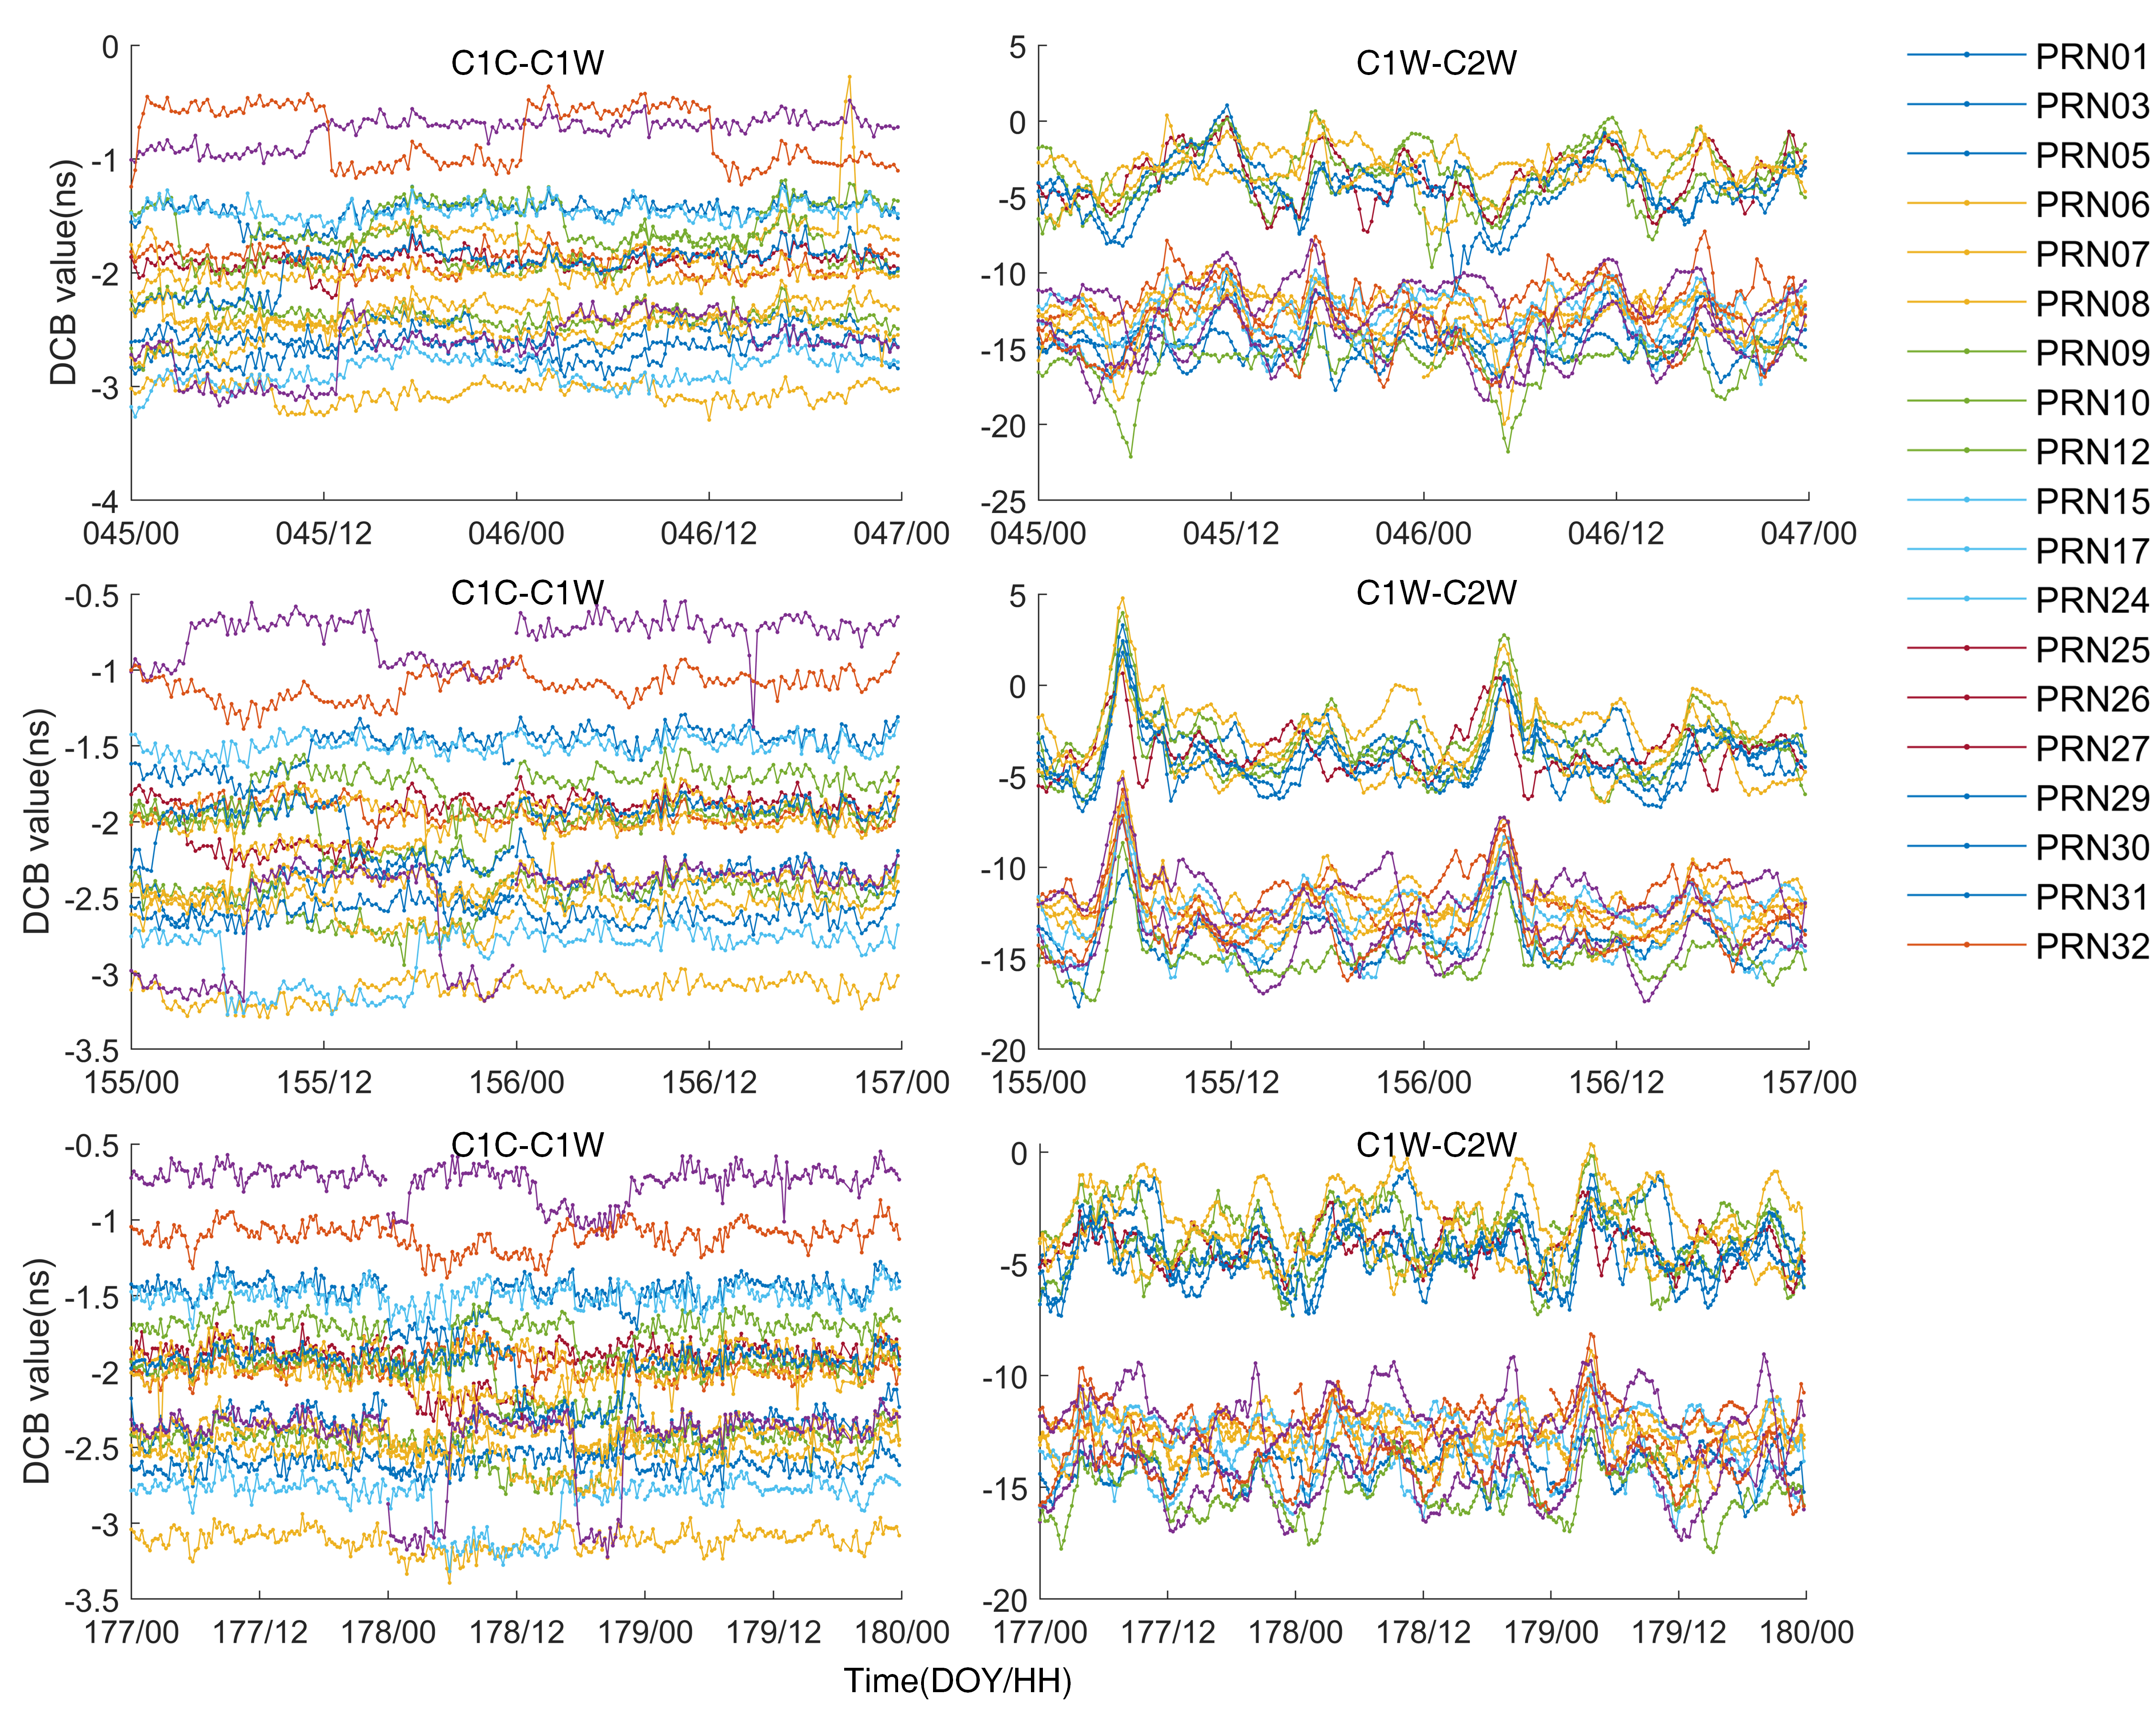
\includegraphics[width=1\linewidth]{figures/c2/dcb/fig6.png}
    \bicaption{2024 年三个弹性功率事件期间,GPS IIR-M 与 IIF 卫星的 C1C–C1W 和 C1W–C2W DCB 估计时间序列。不同颜色的点划线表示不同卫星的 DCB 时间序列,每个点对应一次基于 15 分钟时间窗的估计结果}{Time series of C1C–C1W and C1W–C2W DCB estimates for GPS IIR-M and IIF satellites during three flex power events in 2024. Different colored dash-dot lines represent DCB time series for different satellites, with each point estimated using a 15-min window.}
    \label{fig:dcb_fig6}
\end{figure}

频内 DCB 估计值在多颗卫星上表现出清晰的偏移偏差模式,其偏移持续时间与表 1 中所示的弹性功率激活/停用时间相对应。在这些偏移之外,变化保持稳定在 0.40 ns 以内,且无趋势性行为。相比之下,频间 DCB 估计值未显示出显著的偏移偏差,波动通常控制在 $\pm 6$ ns 以内。频间 DCB 变化在所有三次事件中均表现出 24 小时的周期性,这可能归因于使用 G02 作为参考卫星,其变化模式可能传递给了其他卫星的 DCB 趋势。在事件 2 的频间 DCB 中,两天凌晨 6 点左右出现了显著的数值波动,这可能是由于剧烈的电离层活动所致\cite{ya2010gps}。

图\ref{fig:dcb_fig7}、图\ref{fig:dcb_fig8}以及图\ref{fig:dcb_fig9}说明了三次弹性功率事件期间所有 GPS 卫星的个体 C1C-C1W 频内 DCB 时间序列。在事件 1 期间,除 G05 外的所有 IIR-M 和 IIF 卫星均表现出 DCB 偏移偏差。在事件 2 和 3 期间,所有 IIR-M 和 IIF 卫星均表现出 DCB 偏移偏差。为了调查频内 DCB 偏移偏差是否确实受到弹性功率操作的影响,分析了 2024 年弹性功率事件 3 期间卫星 G32 的多站 S2W C/N0 与 C1C-C1W DCB 估计值之间的关系。图\ref{fig:dcb_fig10}展示了对比时间序列图,其中紫色虚点线代表 C1C-C1W DCB 估计值,彩色圆形标记表示来自多个跟踪站的 S2W C/N0 值。红色和绿色半透明区域分别表示弹性功率的激活和停用时间戳。C1C-C1W DCB 和 C/N0 的阶跃变化之间的时间相关性显而易见,而在其他时段 DCB 值保持稳定在 0.2 ns 范围内。通过系统地比较所有卫星的 DCB 和弹性功率的时间变化,确认了它们的同步发生,证明频内 DCB 偏移确实是由弹性功率操作引起的。
\begin{figure}
    \centering
    \includegraphics[width=1\linewidth]{figures/c2/dcb/fig10.png}
    \bicaption{2024 年弹性功率事件 3 期间,G32 卫星的多站 S2W C/N0 与 C1C–C1W DCB 估计结果对比。紫色点划线表示 C1C–C1W DCB 的时间序列,彩色圆点表示来自多个 MGEX 站的 S2W C/N0 观测值。红色与绿色半透明矩形分别表示弹性功率的开启与关闭时间。可以观察到,C1C–C1W DCB 的跃变与 C/N0 的变化相一致,而在非跃变时段内保持在 0.2 ns 范围内的稳定性,说明 DCB 的变化确实受到弹性功率切换的影响}{Comparison of multi-station S2W C/N0 and C1C–C1W DCB estimation for G32 satellite during flex power event 3 in 2024. The purple dash-dot line represents the C1C–C1W DCB estimation time series, colored circular markers show S2W C/N0 values from multiple MGEX stations. Red and green translucent rectangles indicate flex power on/ off transition timestamps. The shift changes in C1C–C1W DCB coincide with C/N0's shift changes, while maintaining stability within 0.2 ns during other periods, demonstrating that DCB shifts are indeed influenced by flex power changes.}
    \label{fig:dcb_fig10}
\end{figure}

\begin{figure}
    \centering
    \includegraphics[width=0.85\linewidth]{figures/c2/dcb/fig7.png}
    \bicaption{弹性功率事件 1 期间所有 GPS 卫星的 C1C–C1W DCB 估计时间序列}{Time series of C1C–C1W DCB estimates for all GPS satellites during flex power event 1.}
    \label{fig:dcb_fig7}
\end{figure}
\begin{figure}
    \centering
    \includegraphics[width=0.85\linewidth]{figures/c2/dcb/fig8.png}
    \bicaption{弹性功率事件 2 期间所有 GPS 卫星的 C1C–C1W DCB 估计时间序列}{Time series of C1C–C1W DCB estimates for all GPS satellites during flex power event 2.}
    \label{fig:dcb_fig8}
\end{figure}
\begin{figure}
    \centering
    \includegraphics[width=0.85\linewidth]{figures/c2/dcb/fig9.png}
    \bicaption{弹性功率事件 3 期间所有 GPS 卫星的 C1C–C1W DCB 估计时间序列}{Time series of C1C–C1W DCB estimates for all GPS satellites during flex power event 3.}
    \label{fig:dcb_fig9}
\end{figure}
\subsubsection{频间 DCB 变化}

图\ref{fig:dcb_fig11}、图\ref{fig:dcb_fig12}以及图\ref{fig:dcb_fig13}展示了三次弹性功率事件期间所有 GPS 卫星的个体 C1W-C2W 频间 DCB 时间序列。在这些事件中未检测到 DCB 值的偏移偏差,这表明在当前的噪声估计水平下,无法确定弹性功率对频间 DCB 的影响。虽然各事件间的日内 DCB 变化模式有所不同,但在每个事件中都观察到了明显的日周期性,这可能归因于电离层活动变化。此外,使用 G02 作为参考卫星必然会将 $sDCB_{G02}$ 值趋向于零。然而,由于 sDCB 可能会经历日内变化,G02 卫星行为的变化可能会在其他卫星的 DCB 估计结果中显现出来。

\begin{figure}
    \centering
    \includegraphics[width=0.85\linewidth]{figures/c2/dcb/fig11.png}
    \bicaption{弹性功率事件1期间所有GPS卫星的C1W–C2W DCB估计时间序列}{Time series of C1W–C2W DCB estimates for all GPS satellites during flex power event 1.}
    \label{fig:dcb_fig11}
\end{figure}

\begin{figure}
    \centering
    \includegraphics[width=0.85\linewidth]{figures/c2/dcb/fig12.png}
    \bicaption{弹性功率事件2期间所有GPS卫星的C1W–C2W DCB估计时间序列}{Time series of C1W–C2W DCB estimates for all GPS satellites during flex power event 2.}
    \label{fig:dcb_fig12}
\end{figure}

\begin{figure}
    \centering
    \includegraphics[width=0.85\linewidth]{figures/c2/dcb/fig13.png}
    \bicaption{弹性功率事件3期间所有GPS卫星的C1W–C2W DCB估计时间序列}{Time series of C1W–C2W DCB estimates for all GPS satellites during flex power event 3.}
    \label{fig:dcb_fig13}
\end{figure}

\section{本章小结}
弹性功率是GNSS现代化进程中一项关键的抗干扰技术,通过在不同信号分量间重分配发射功率,直接改变了信号的物理特性。本章首先梳理了弹性功率的定义与发展历程,详细分析了从区域性增强到全球模式演变的十种运行模式,并通过二维轨迹与三维投影的可视化手段展示了其覆盖特征。针对C/N0受到的影响,归纳出“阶跃提升”和“整体提升”两种典型模式,并结合卫星轨迹提出了无需依赖特定阈值的可视化方法。实验表明,不同接收机-天线组合对弹性功率的响应存在显著的系统性差异,最大偏差可达 2.56 dB-Hz,这说明依赖单一基线模型的检测方法存在局限性,需建立更具普适性的检测策略。

弹性功率的激活会导致卫星通道硬件延迟在日内发生显著跳变,传统的单日均值估计策略已不再适用。为了捕捉这一短时变化特征,提出了基于 15 分钟滑动窗口的短期 DCB 估计算法。该方法联合估计电离层球谐系数与硬件偏差,并采用内符合精度作为质量控制指标。最终,利用 2024 年三次典型的弹性功率事件,量化评估了弹性功率对 GPS 卫星频内与频间 DCB 的具体影响。实验结果显示,频内 DCB(C1C-C1W)呈现出约 0.4 ns 的系统性偏移,且该偏移与 C/N0 的阶跃变化具有严格的时间同步性,估计结果的 RMS 优于 0.0075 ns;而频间 DCB(C1W-C2W)在现有估计精度下未表现出明显的阶跃特征,主要受电离层活动影响呈现周日周期性波动。上述结论证实了弹性功率是引起观测值异常和硬件偏差不稳定的重要物理诱因,若在高精度数据处理中不予修正,将直接制约定位性能。